\documentclass{beamer} \usetheme{Madrid}
\usecolortheme{beaver}

\setbeamertemplate{enumerate items}[circle]
\setbeamercolor{item projected}{bg=red!70!black}

\usepackage[utf8]{inputenc}
\usepackage{mdframed}
\usepackage{minted}
\usepackage{tikz}
\usetikzlibrary{shapes.geometric, arrows}

\tikzstyle{node} = [rectangle, minimum width=7mm, minimum height=7mm, text centered, fill=gray!30]
\tikzstyle{arrow} = [thick,->,>=stealth]

\newenvironment{question}[1][]{
    \ifstrempty{#1}{}
    {\mdfsetup{
        frametitle={
            \tikz[baseline=(current bounding box.east),outer sep=0pt]
            \node[anchor=east,rectangle,fill=gray!30]
            {#1};
        }
    }}
    \mdfsetup{
        innertopmargin=10pt,linecolor=gray!30,
        linewidth=2pt,topline=true,
        frametitleaboveskip=\dimexpr - \ht\strutbox\relax
    }
    \begin{mdframed}
}{
    \end{mdframed}
}

\title{Linux Workshop}
\subtitle{Spring 2022}

\author[]{Jack Leightcap\inst{1}\inst{2}, Connor Northway\inst{2}}

\institute[IEEE, Wireless Club]{
    \inst{1}IEEE -- \url{nuieeeofficers@gmail.com}
    \and
    \inst{2}Wireless Club -- \url{nuwirelessclub@gmail.com}
}

\date[Spring 2022]{February 7, 2022}

\begin{document}
\frame{\titlepage}

\begin{frame}
    \frametitle{What is Linux?}
    \begin{columns}
        \begin{column}{0.6\textwidth}
            \begin{itemize}
                \item Free and open source -- \url{https://github.com/torvalds/linux}
                \item Source code makes debugging and extending (comparatively!) easy
                \item Modular, configurable: small low power systems to large complex systems
                \item 10,000+ contributors, regular release cycle
                \item Linus's Law - ``given enough eyeballs, all bugs are shallow''
            \end{itemize}
        \end{column}
        \begin{column}{0.4\textwidth}
            \centering
            \begin{figure}
                
\includegraphics[width=0.4\textwidth]{tux.png}
                \caption{Tux, Linux Mascot}
            \end{figure}
        \end{column}
    \end{columns}
\end{frame}

\begin{frame}
    \frametitle{The UNIX Philosophy}
    \vfill
    Peter H. Salus, \emph{A Quarter-Century of Unix}, from Doug McIlroy;
    \begin{itemize}
        \item Write programs that do one thing and do it well.
        \item Write programs that work together.
        \item Write programs to handle text streams, because that is the universal interface.
    \end{itemize}
    \vspace{1cm}
    Opposed to \emph{Zawinski's Law}:
    \begin{itemize}
        \item Every program attempts to expand until it can read [e]mail.
            Those programs which cannot so expand are replaced by ones which can.
    \end{itemize}
    \vfill
\end{frame}

\begin{frame}
    \vfill
    \begin{center}
    \begin{figure}
        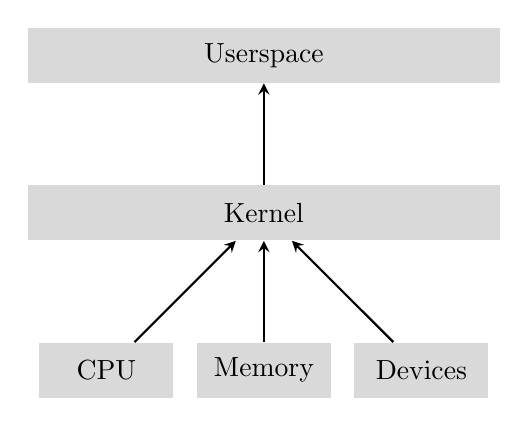
\begin{tikzpicture}[node distance=2cm]
            \node (uspace) [node, minimum width=6cm] {Userspace};
            \node (kspace) [node, minimum width=6cm, below of=uspace] {Kernel};
            \node (mem)    [node, minimum width=17mm, below of=kspace] {Memory};
            \node (cpu)    [node, minimum width=17mm, left of=mem] {CPU};
            \node (hard)   [node, minimum width=17mm, right of=mem] {Devices};

            \draw [arrow] (kspace) -- (uspace);
            \draw [arrow] (cpu)    -- (kspace);
            \draw [arrow] (mem)    -- (kspace);
            \draw [arrow] (hard)   -- (kspace);
        \end{tikzpicture}
        \caption{General System Hierarchy}
    \end{figure}
    \end{center}
    \vfill
\end{frame}

\begin{frame}
    \begin{figure}
        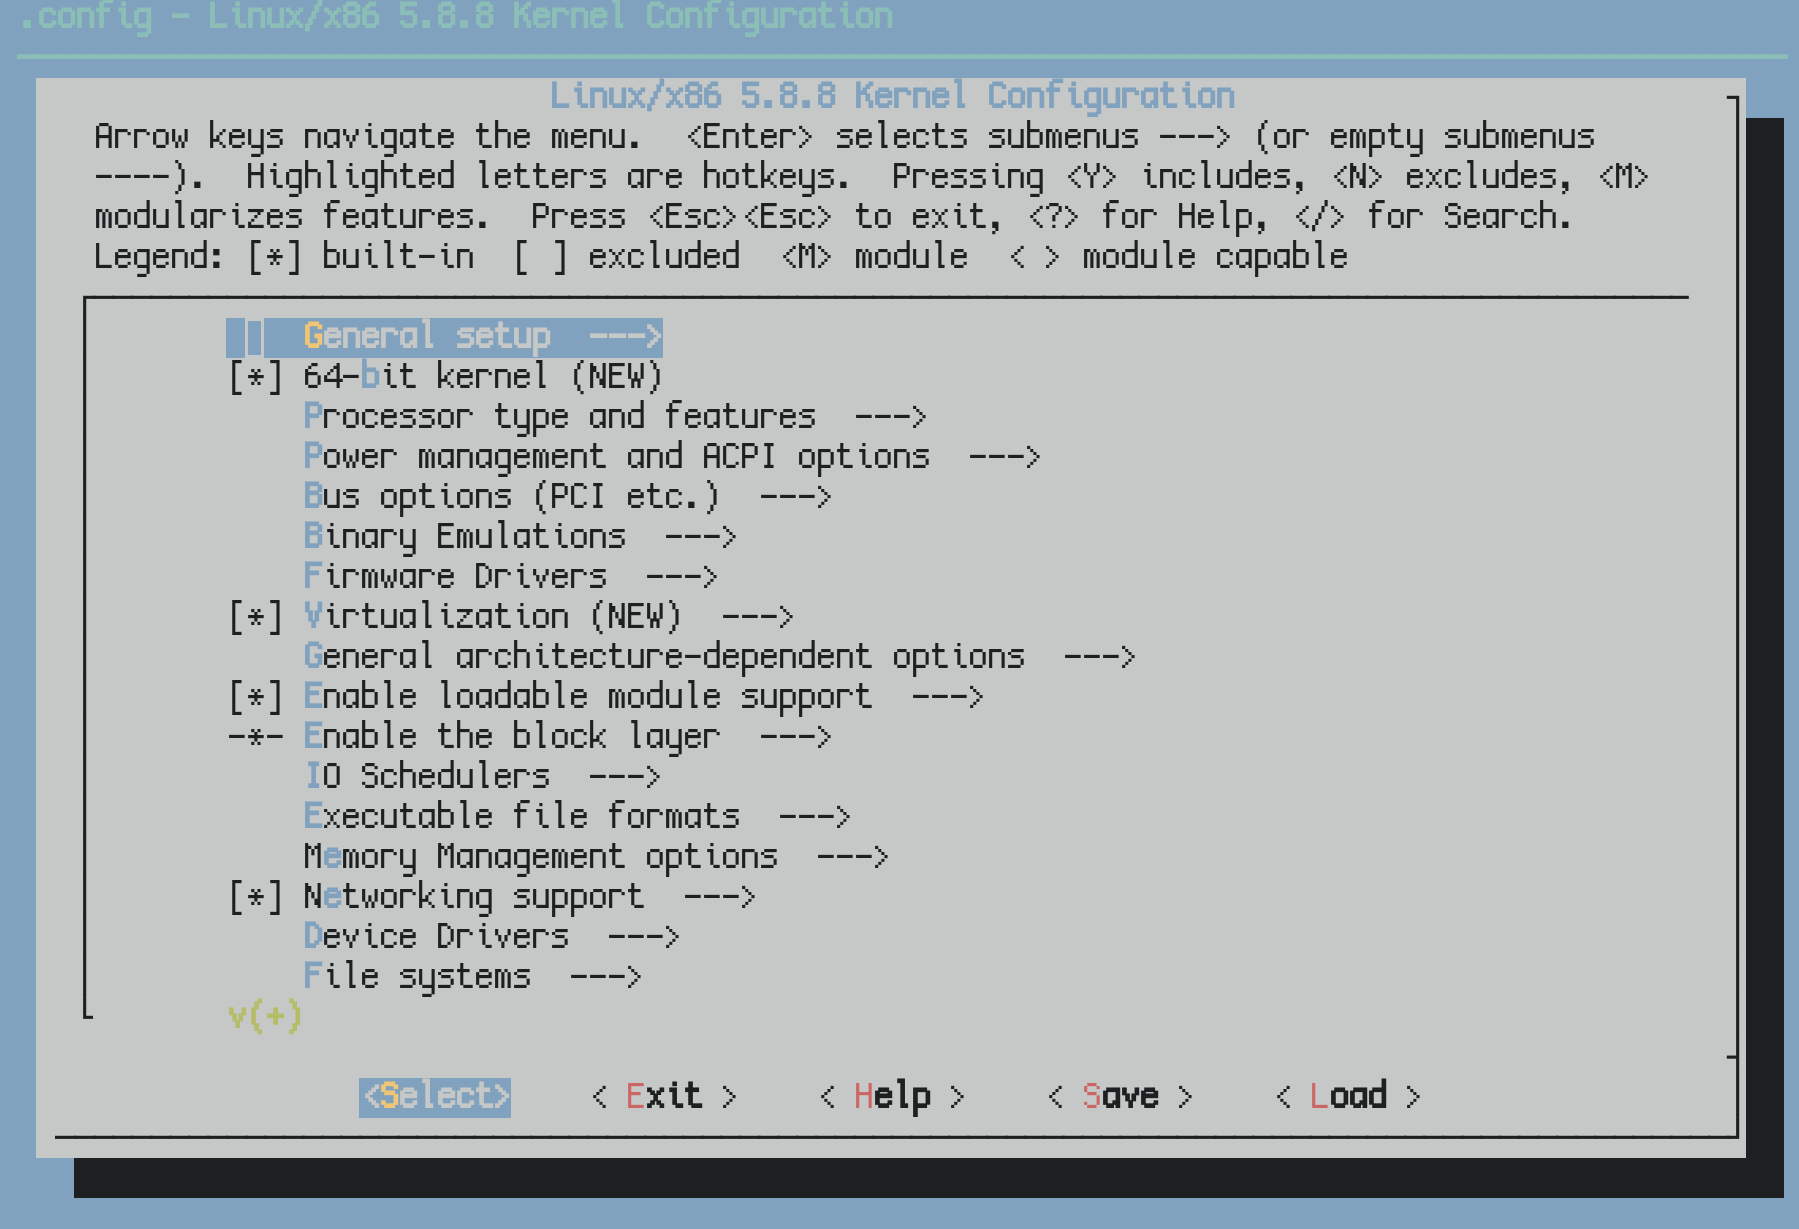
\includegraphics[width=10cm]{menuconfig.png}
        \caption{\texttt{menuconfig} -- Linux configuration}
    \end{figure}
\end{frame}

\begin{frame}
    \frametitle{What is Linux Used For?}
    \begin{center}
        From `big' to `small':
        \begin{itemize}
            \item Servers (`The Cloud')
            \item Supercomputers
            \item Personal computers
            \item Android
            \item IoT Devices
            \item Embedded Systems
        \end{itemize}
        And almost everything in between
    \end{center}
\end{frame}

\begin{frame}
    \begin{figure}
        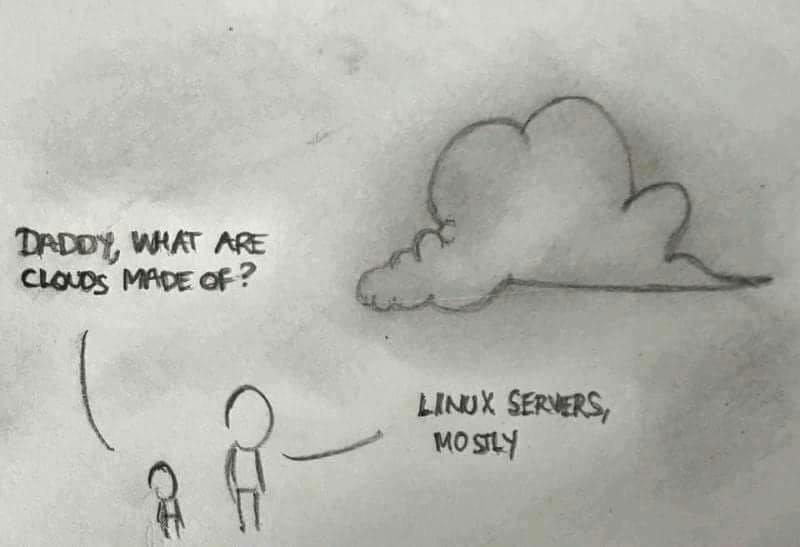
\includegraphics[width=10cm]{cloud.jpg}
        \caption{\href{https://www.reddit.com/r/ProgrammerHumor/comments/6cer5t/what_are_clouds_made_of/}{Source}}
    \end{figure}
\end{frame}

\begin{frame}
    \begin{figure}
        \includegraphics[width=10cm]{businesscard-top.jpg}
        \caption{\href{https://www.thirtythreeforty.net/posts/2019/12/designing-my-linux-business-card/}{Source}}
    \end{figure}
\end{frame}

\begin{frame}
    \begin{figure}
        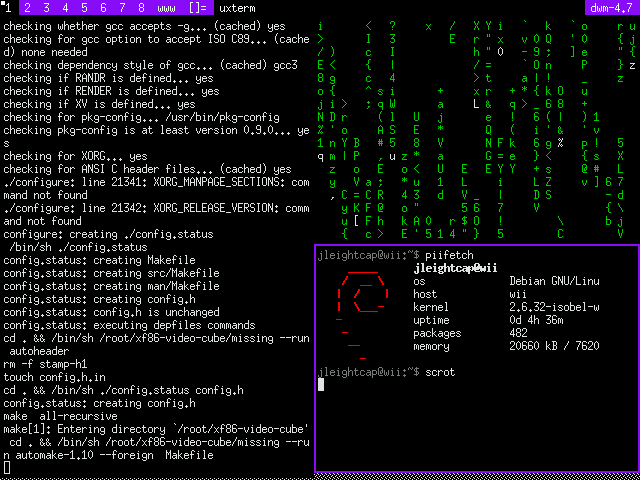
\includegraphics[width=10cm]{wiilinux.png}
        \caption{\href{http://www.gc-linux.org/wiki/WL:whiite-linux}{Source}}
    \end{figure}
\end{frame}

\begin{frame}{Booting Linux in Web Browser}
    \vfill
        Ideally in another window,
        \center{\Large{\url{http://copy.sh/v86/?profile=linux26}}}
    \vfill
\end{frame}

\begin{frame}{Interacting with Linux: the shell}
    \begin{itemize}
        \item The \emph{shell} is a text-based interface to the kernel
        \item a \emph{REPL} (Read $\rightarrow$ Eval $\rightarrow$ Print $\rightarrow$ Loop) of a complete programming language; loops, variables, etc.
    \end{itemize}
    \vspace{7mm}
    After booted:\\[5mm]
    \begin{tabular}{ll}
        \textbf{/root\% pwd} \hspace{15mm} & \texttt{pwd} -- ``Print Working Directory''\\
        \texttt{/root} \\
        \textbf{/root\% cd /} & \texttt{cd} -- ``Change Directory''\\
        \textbf{/\% ls} & \texttt{ls} -- ``List'' \\
        ...
    \end{tabular}
\end{frame}

\begin{frame}
    \frametitle{Filesystem Organization}
    \begin{center}
    \begin{figure}
        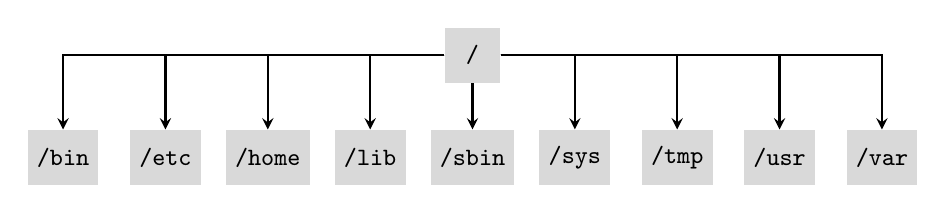
\begin{tikzpicture}[node distance=13mm]
            \node (bin)  [node] {\small\texttt{/bin}};
            \node (etc)  [node, right of=bin]  {\small\texttt{/etc}};
            \node (home) [node, right of=etc]  {\small\texttt{/home}};
            \node (lib)  [node, right of=home] {\small\texttt{/lib}};
            \node (sbin) [node, right of=lib]  {\small\texttt{/sbin}};
            \node (sys)  [node, right of=sbin] {\small\texttt{/sys}};
            \node (tmp)  [node, right of=sys]  {\small\texttt{/tmp}};
            \node (usr)  [node, right of=tmp]  {\small\texttt{/usr}};
            \node (var)  [node, right of=usr]  {\small\texttt{/var}};
            \node (root) [node, above of=sbin] {\small\texttt{/}};

            \draw [arrow] (root) -| (bin);
            \draw [arrow] (root) -| (etc);
            \draw [arrow] (root) -| (home);
            \draw [arrow] (root) -| (lib);
            \draw [arrow] (root) -- (sbin);
            \draw [arrow] (root) -| (sys);
            \draw [arrow] (root) -| (tmp);
            \draw [arrow] (root) -| (usr);
            \draw [arrow] (root) -| (var);
        \end{tikzpicture}
        \caption{Common Linux Directory Structure}
        \end{figure}
        \vspace{1cm}
        \begin{tabular}{l|l}
            shorthand & meaning \\
            \hline
            \texttt{.}  & current directory \\
            \texttt{..} & parent (upper) directory \\
            \texttt{\~} & home directory
        \end{tabular}
    \end{center}
\end{frame}

\begin{frame}
    \begin{question}[\emph{QUESTION}: Parent Directory of \texttt{/}]
        \texttt{/\% pwd}\\
        \texttt{/}\\
        \texttt{/\% cd ..}\\[3mm]
        where are we?
    \end{question}
\end{frame}

\begin{frame}
    \frametitle{Special Directories: \texttt{/dev}, \texttt{/proc}, and \texttt{/tmp}}
    \center{``[text streams are] the universal interface``} -- everything is a file!
    \vspace{1cm}
    \begin{itemize}
        \item \texttt{/dev/}: devices
            \begin{itemize}
                \item Random numbers: \texttt{/dev/urandom}
                \item Zero: \texttt{/dev/zero} (surprisingly useful)
                \item Physical storage: \texttt{/dev/hda}, \texttt{/dev/sda}, ...
                \item RAM: \texttt{/dev/ram}
            \end{itemize}
        \item \texttt{/proc/}: processes
            \begin{itemize}
                \item CPU info: \texttt{cat /proc/cpuinfo}
                \item Linux version info: \texttt{cat /proc/version}
                \item Processes: \texttt{ps} PIDs compared to \texttt{ls /proc}
            \end{itemize}
        \item \texttt{/tmp/}: temporary (sometimes cleared on reboot)
    \end{itemize}
\end{frame}

\begin{frame}
    \frametitle{\texttt{/bin}, \texttt{/sbin}, \texttt{/usr/bin}, and \texttt{/usr/sbin}: Programs}
    \begin{itemize}
        \item \texttt{ls /bin} --- see \texttt{ls} there?
        \item How does the system know where to look for these? Similar to other programming langages, a \emph{variable}:
            \begin{itemize}
                \item \texttt{FOO=hello}, get contents of variable with \texttt{echo \$FOO}
                \item \texttt{echo \$PATH}
                \item Have programs in \texttt{/root}? \texttt{PATH=\$PATH:/root}
            \end{itemize}
        \item Layout has standards, but in the end up to user
            \begin{itemize}
                \item \emph{symlinks} -- ``Symbolic Links'' have one file or directory `point' to another
                \item \texttt{/usr/local/bin}, programs will change default \texttt{\$PATH}, plenty of others\ldots
            \end{itemize}
    \end{itemize}
\end{frame}

\begin{frame}
    \frametitle{Shell Extras}
    \begin{itemize}
        \item \texttt{[COMMAND] > file} \\ write output of \texttt{[COMMAND]} to \texttt{file}
        \item \texttt{[COMMAND]$_1$ | [COMMAND]$_2$ | ...} \\ \emph{pipe} output of one command to the input of the next
        \item \texttt{[COMMAND] \&} \\ run \texttt{[COMMAND]} in the background.
        \item \texttt{foo() \{ [COMMAND] \}} \\ define a function \texttt{foo} which does \texttt{[COMMAND]}.
    \end{itemize}
    Piping examples:
    \begin{itemize}
        \item \texttt{ls /bin | sort | head -n 1} \\ first program in bin, alphabetically
        \item \texttt{cat /root/tests/reference.test | uniq | wc -l} \\ last program in bin, alphabetically
    \end{itemize}
\end{frame}

\begin{frame}
    \begin{question}[NOTE: What Do These Do?]
        \texttt{/\% fork() \{ fork | fork \& \}}\\
        \texttt{/\% fork}\\[1cm]
        \texttt{/\% rm -r /}
    \end{question}
\end{frame}

\begin{frame}
    \frametitle{Power and Responsibility...}
    \begin{center}
        \emph{Linux gives you the power to shoot yourself in the foot.}
    \end{center}
    General precautions:

    \begin{itemize}
        \item Don't copy paste a shell command without understanding what it's doing.
        \item Don't run a script from an untrusted source without verifying it.
        \item Easy mistakes that can permanently delete files:
            \begin{itemize}
                \item Moving file over another
                \item Writing over a file
                \item Over-reliance on tab completion
                \item There is no recycling bin in the shell!
            \end{itemize}
    \end{itemize}
\end{frame}

\end{document}
